% !TEX program = lualatex
\documentclass[french,a4paper]{article}

\usepackage{amsmath,amsthm,amssymb}
\usepackage{fontspec}
%\usepackage{unicode-math}
\defaultfontfeatures{Ligatures=Common}
\setmainfont{Cambria}
\setsansfont{Calibri}
\setmonofont{Consolas}[Scale=MatchLowercase]

\usepackage{stmaryrd}
\usepackage{polyglossia}
\usepackage{enumitem}
\usepackage{tikz,tikz-cd}
\usepackage[explicit]{titlesec}
\usepackage{listings}
\usepackage{hyperref}
\usepackage{fmtcount}
\usepackage{microtype} % uncomment for better rendering
\usepackage{titlepage}

\usetikzlibrary{decorations.markings}

\setmainlanguage{french}
\setlist[itemize]{label=--}

\lstdefinestyle{sh}{%
  language=sh,%
  basicstyle=\tt\small,%
}
\lstdefinestyle{C}{%
  language=C,%
  breaklines=true,%
  frame=l,%
  xleftmargin=\parindent,%
  basicstyle=\ttfamily\small,%
  keywordstyle=\bfseries\color{green!40!black!80},%
  showstringspaces=false,%
  commentstyle=\itshape\color{purple!70},%
  identifierstyle=\color{blue!80},%
  stringstyle=\color{red!80},%
  directivestyle=\color{orange!90!black!80},%
  % otherkeywords={},%
  escapeinside={<latex>}{</latex>},%
}
\lstset{style=C}


\title{Projet de programmation en {\tt C}:\\
  solveur de sudoku}
\date{\`A rendre pour le 14 janvier 2017}
\author{}
\otherauthor{Pierre Cagne}
\conf{%
  {\Large UGMT41 --- Algorithmique et Projet de programmation}%
}
\subconf{%
  \begin{minipage}{.8\linewidth}\flushright
    Master 1 de Mathématiques et applications\\
    Université Paris Diderot
  \end{minipage}%
}
\mail{pierre.cagne@normalesup.org}
\license{Licensed under CC-BY-SA 4.0 International}
\bgcolor{green!40!black!80}
\logo{ex-sudoku.png}

\theoremstyle{definition}
\newtheorem{exercise}{Exercice}
\newtheorem{question}{Question}
\newtheorem*{definition}{Définition}
\theoremstyle{remark}
\newtheorem*{remark}{Remarque}
\newtheorem*{examples}{Exemples}

\newcommand{\shell}[1]{\lstinline[style={},style=sh]|#1|}
\newcommand{\inlinec}[1]{\lstinline[style=C]°#1°}

\DeclareMathOperator{\powersetoperator}{\mathcal P}
\newcommand{\powerset}[1]{\powersetoperator(#1)}

\begin{document}

\begin{abstract}
  Ce projet de programmation a pour but de vous faire coder un solveur
  du jeu de sudoku par des méthodes avancées de {\em backtracking}. Ce
  domaine de l'algorithmique est dévoué à l'étude des méthodes de
  recherche exhaustive de solutions à un problème donné en évitant
  tant que possible la méthode dite de {\em brute-force} (qui consiste
  à essayer toutes les possibilités pour en extraire les solutions).
\end{abstract}

\maketitle

%%% main matter

L'implémentation d'un solveur de sudoku peut prendre différentes
formes. L'idée la plus simple serait de tester toutes les combinaisons
possibles de remplissage de la grille et de ne garder que celle(s)
satisfaisant aux règles classiques du sudoku: un unique $i$ par ligne,
colonne et bloc pour $i \in \{1,\dots,9\}$. C'est ce que l'on appelle
la méthode {\em brute-force}: elle teste les $m^9$ remplissages
possibles, $m$ étant le nombre de cases vides de la grille
(typiquement $m$ est de l'ordre de $60$ à $65$), y compris les
remplissages les plus stupides, avec par exemple deux $1$ l'un
à côté de l'autre... Autant dire qu'il y a de la place pour améliorer
cela!

Le but de ce projet est de vous faire implémenter un solveur plus
efficace grâce à un processus en trois étapes\footnote{C'est un
  processus que vous pouvez appliquer à la plupart des problèmes
  concrets que vous souhaitez résoudre informatiquement.}: une
modélisation mathématique abstraite du problème à résoudre; un
traitement algorithmique du problème abstrait ; une implémentation
efficace de l'algorithme, grâce aux outils du langage à
disposition. Bien entendu, on n'attend pas de vous que vous fassiez
tout cela tout seul, et les trois premières parties de ce document
sont justement là pour vous guider.

La première étape, en section \ref{sec:exact-hit}, peut sembler à
première vue complexifier le problème. En fait, en incluant le sudoku
dans une classe plus large de «~puzzles~», on identifie précisément ce
qui fait la complexité de la résolution d'une grille de sudoku. La
deuxième étape, présentée en section \ref{sec:algo-sol}, va permettre
d'encoder les notions abstraites de la première étape comme des objets
concrets, afin de concevoir un algorithme efficace résolvant le
problème. Enfin, la troisième étape, en section \ref{sec:dlx}, vous
invite à utliser tous les outils mis à votre disposition par le
langage {\tt C} pour coder effectivement les objets et l'algorithme
pensés à la deuxième étape. La section \ref{sec:actual-project}
détaille les modalités de rendu du projet.

\begin{remark}
  Les trois premières parties doivent se lire avec un papier et un
  stylo à la main, et {\bf surtout pas} avec un clavier et un fichier
  \shell{.c} ouvert à l'écran...
\end{remark}

\medskip

Dans tout le document, on fait l'hypothèse que l'on ne manipule que
des ensembles {\em finis}.

\section{Problème de satisfaction de contraintes}
\label{sec:exact-hit}

Supposons qu'on ait deux ensembles $P$ et $C$ et une relation
$\mathcal S \subseteq P \times C$. On appelera les éléments de $P$ des
{\em possibilités} et ceux de $C$ des {\em contraintes}. Comme
d'habitude, on notera $p \mathrel{\mathcal S} c$ plutôt que
$(p,c) \in \mathcal S$ pour des éléments $p\in P$ et $c\in C$, et on
dira dans ce cas que {\em $p$ satisfait la contrainte $c$}.

\begin{definition}
  Un tel triplet $(P,C,\mathcal S)$ est appelé {\em problème de
    satisfaction de contraintes}.

  Une {\em solution} du problème $(P,C,\mathcal S)$ est un
  sous-ensemble $P^\ast \subseteq P$ tel que toute contrainte
  $c \in C$ soit satisfaite par {\bf exactement une} possibilité
  $p \in P^\ast$. Autrement dit, c'est une fonction $f : C \to P$
  telle que $f(c) \mathrel{\mathcal S} c$ pour tout $c \in C$.
\end{definition}

\begin{remark}
  Attention, le vocabulaire utilisé dans ce document est hautement
  {\bf non standard}. En particulier, googliser «~problème de
  satisfaction de contraintes~» ou «~constraint satisfaction problem~»
  risque de vous emmener vers des considérations mathématiques et
  algorithmiques qui n'ont que très peu à voir avec les notions
  présentées ici.
\end{remark}

Malgré son apparente abstraction, la notion de problème de
satisfaction de contraintes est omniprésente, en mathématiques comme
dans la vie courante. En voici quelques exemples.
\begin{examples}~
  \begin{enumerate}[label=(\arabic*)]
  \item Soit $X$ un ensemble. Les solutions au problème de
    satisfaction de contraintes $(\powerset X, X, \ni)$ sont
    exactement les partitions de $X$.
  \item On trouve souvent des problèmes de satisfaction de contraintes
    dans les revues de divertissement sous forme de «~puzzles
    logiques~». Ce sont ces problèmes logiques posés sous la forme
    suivante:
    \begin{center}
      \begin{minipage}{0.8\linewidth}
        Alice, Bob et Dave ont fait des emplettes. L'un a acheté des
        carottes, un autre des pommes de terres et le dernier des
        oignons. Ils ont fait leurs achats chacun différemment: en
        grande surface, au marché ou chez l'épicier. Retrouver qui à
        acheter quoi et où, sachant que:
        \begin{enumerate}[label=($C_{\arabic*}$)]
        \item Alice n'aime pas la grande distribution,
        \item L'épicier n'avait plus de carottes,
        \item Les pommes de terre ont été achetés au marché,
        \item L'un de Bob ou Dave est allé chez l'épicier,
        \item Dave déteste les oignons.
        \end{enumerate}
      \end{minipage}
    \end{center}
    On peut modéliser le puzzle comme un problème de satisfaction de
    contraintes: l'ensemble $P$ des possibilités sont les triplets
    $(\mathrm{nom},\mathrm{produit},\mathrm{lieu})$ et l'ensemble $C$
    des contraintes est donné par $\{C_1,C_2,C_3,C_4,C_5\}$ auquel on
    ajoute les contraintes implicites du problème: une contrainte par
    nom (notons les $A$ pour Alice, $B$ pour Bob et $D$ pour Dave),
    une par produit ($c$ pour carottes, $p$ pour pommes de terre, et
    $o$ pour oignons), et une par lieu ($e$ pour épicier, $m$ pour
    marché et $s$ pour supermarché). Bien entendu, la relation
    $\mathcal S$ de satisfaction est définie comme la satisfaction de
    la contrainte au sens courant du terme: par exemple,
    \begin{displaymath}
      \begin{aligned}
        (\mathrm{Alice},\mathrm{oignons},\mathrm{supermarché})
        &\mathrel{\mathcal S} A, \\
        % 
        (\mathrm{Alice},\mathrm{carottes},\mathrm{supermarché})
        &\mathrel{\not \kern-2pt\mathcal S} C_1, \\
        % 
        (\mathrm{Bob},\mathrm{pommes\ de\ terre},\mathrm{épicier})
        &\mathrel{\mathcal S} C_4, \quad\text{etc.}
      \end{aligned}
    \end{displaymath}
    Dans le cas présent (et dans la plupart des puzzles de ce genre),
    il y a une unique solution au problème de satisfaction de
    contraintes.
  \item Supposons qu'un maçon veuille paver la cour d'un jardin
    (représentée à gauche) avec des tuiles toutes de la même forme
    (représentée à droite):

    \begin{minipage}{.68\textwidth}\centering
      \begin{tikzpicture}[scale=.7]
        \draw[dotted] (0,0) grid (6,6);%
        \draw[thick] (0,0) -- (6,0) -- (6,6) -- (0,6) -- cycle;%
      \end{tikzpicture}
    \end{minipage}
    \begin{minipage}{.3\textwidth}\flushleft
      \begin{tikzpicture}[scale=.7]
        \draw[fill=lightgray] (0,0) -- (2,0) -- (2,1) -- (1,1)
        -- (1,2) -- (0,2) -- cycle;%        
        \draw[dotted] (1,0) -- (1,1) -- (0,1);%
      \end{tikzpicture}
    \end{minipage}

    Il a le droit de placer les tuiles dans le sens qu'il veut et où
    il veut dans la cour, mais à la fin les tuiles ne doivent pas se
    superposer et chaque carré de la cour doit être couvert.
    
    Pour énumérer toutes les possibilités et choisir parmi celles-ci,
    il peut modéliser la situation comme un problème de satisfaction
    de contraintes comme suit: l'ensemble $P$ des possibilités est
    l'ensemble des triplets $(x_1,x_2,x_3)$ avec
    $x_1,x_2,x_3 \in [1,6]\times[1,6]$ d'une des formes suivantes:
    \begin{displaymath}
      \begin{aligned}
        ((i,j+1),(i,j),(i+1,j)) &\qquad
        ((i,j-1),(i,j),(i+1,j))\\
        ((i,j-1),(i,j),(i-1,j)) &\qquad
        ((i,j+1),(i,j),(i-1,j))
      \end{aligned}
    \end{displaymath}
    C'est-à-dire que $P$ est l'ensemble des placements possibles de la
    tuile (rotations comprises) dans la cour. L'ensemble $C$ des
    contraintes est $[1,6] \times [1,6]$, c'est-à-dire l'ensemble des
    carrés de la cour. La relation de satisfaction, définie par
    \begin{displaymath}
      (x_1,x_2,x_3) \mathrel{\mathcal S} c \iff \exists i,\, x_i = c,
    \end{displaymath}
    exprime alors simplement le fait qu'un carré $c$ est recouvert par
    le placement en $(x_1,x_2,x_3)$ de la tuile. Une solution au
    problème $(P,C,\mathcal S)$ est donc la sélection $P^\ast$ d'un
    certain nombres de placements de tuiles de telle sorte que chaque
    carré de la cour soit recouvert par exactement une tuile de
    $P^\ast$: c'est bien la définition d'un pavage de la cour. Par
    exemple, on a la solution suivante (bien entendu, ce n'est pas la
    seule) représentée graphiquement en figure \ref{fig:tiling}:
    \begin{displaymath}
      P^\ast = \left\{
        \begin{aligned}
          &((1,2),(1,1),(2,1)),\,
          ((4,2),(4,1),(5,1)),\,
          ((1,4),(1,3),(2,3)),\\
          &((4,4),(4,3),(5,3)),\,
          ((1,6),(1,5),(2,5)),\,
          ((4,6),(4,5),(5,5)),\,\\
          &((2,2),(3,2),(3,1)),\,
          ((5,2),(6,2),(6,1)),\,
          ((2,4),(3,4),(3,3)),\\
          &((5,4),(6,4),(6,3)),\,
          ((2,6),(3,6),(3,5)),\,
          ((5,6),(6,6),(6,5))
        \end{aligned}
      \right\}
    \end{displaymath}
    \begin{figure}[h!]
      \centering %
      \begin{tikzpicture}[scale=.7]
        \fill[lightgray] (0,0) rectangle (6,6);%
        \draw[dotted] (0,0) grid (6,6);%
        \draw[thick] (0,0) -- (6,0) -- (6,6) -- (0,6) -- cycle;%
        \draw (0,2) -- (6,2);%
        \draw (0,4) -- (6,4);%
        \draw (3,0) -- (3,6);%
        \draw (1,2) -- ++(0,-1) -- ++(1,0) -- ++(0,-1);%
        \draw (4,2) -- ++(0,-1) -- ++(1,0) -- ++(0,-1);%
        \draw (1,4) -- ++(0,-1) -- ++(1,0) -- ++(0,-1);%
        \draw (4,4) -- ++(0,-1) -- ++(1,0) -- ++(0,-1);%
        \draw (1,6) -- ++(0,-1) -- ++(1,0) -- ++(0,-1);%
        \draw (4,6) -- ++(0,-1) -- ++(1,0) -- ++(0,-1);%
      \end{tikzpicture}%
      \caption{Exemple de pavage}%
      \label{fig:tiling}%
    \end{figure}
  \end{enumerate}
\end{examples}

\begin{question}
  Montrer que le jeu de sudoku est un problème de satisfaction de
  contraintes. Plus exactement, si $G$ est une grille de sudoku,
  contruire un problème $(P_G,C_G,\mathcal S_G)$ de telle façon que
  les solutions $P_G^\ast$ soient (en bijection avec) les remplissages
  valides de la grille $G$.
\end{question}

\section{Résolution algorithmique}
\label{sec:algo-sol}%

La question suivante permet de reformuler les problèmes de
satisfaction de contraintes dans un langage plus adapté à
l'implémentation en {\tt C}.

\begin{question}
  Soit $(P,C,\mathcal S)$ un problème de satisfaction de
  contraintes. Constuire une matrice
  $M = (m_{i,j})_{1\leq i \leq p,1\leq j\leq q}$ (à vous de trouver
  $p$ et $q$) à coefficients $m_{i,j} \in \{0,1\}$ de telle façon que
  les solutions du problème $(P,C,\mathcal S)$ soient en bijection
  avec l'ensemble
  \begin{displaymath}
    \left\{
      (i_1,i_2,\dots,i_n) \middle| 
      \begin{pmatrix}
        m_{i_1,1} & m_{i_1,2} & \dots & m_{i_1,q} \\
        m_{i_2,1} & m_{i_2,2} & \dots & m_{i_2,q} \\
        \vdots & \vdots & \ddots & \vdots \\
        m_{i_n,1} & m_{i_n,2} & \dots & m_{i_n,q}
      \end{pmatrix} \
      \text{a exactement un $1$ par colonne}
    \right\}
  \end{displaymath}
  \`A partir de maintenant, on appelle donc aussi {\em solution} du
  problème un tel uplet $(i_1,\dots,i_n)$, et on dira que la matrice
  $M$ {\em présente} le problème $(P,C,\mathcal S)$.
\end{question}

La question de trouver toutes les solutions d'un problème de
satisfaction de contraintes est donc maintenant ramenée à
l'élaboration d'un algorithme déterminant toutes les sélections de
lignes possibles d'une matrice à coefficients booléens (i.e.\ dans
$\{0,1\}$) de telle manière que la matrice résultante ait un unique
$1$ dans chaque colonne.

\begin{question}
  \label{question:recursive-matrix}%
  Remarquer qu'une solution contenant une ligne fixée est exactement
  la même chose qu'une solution d'un problème plus restreint. Plus
  précisément, si on fixe une ligne $i$, une solution
  $(i_1,\dots,i_n)$ du problème présenté par $M$ pour laquelle $i_k=i$
  est exactement la donnée d'une solution
  $(i_1,\dots,i_{k-1},i_{k+1},\dots,i_n)$ pour le problème présenté
  par la matrice obtenue à partir de $M$ comme suit:
  \begin{itemize}
  \item on choisit un colonne $j$ pour laquelle la ligne $i$ a un $1$,
  \item on enlève toute les lignes de $M$ qui ont un $1$ dans cette
    colonne $j$,
  \item on enlève également la colonne $j$.
  \end{itemize}

  \`A partir de cette observation, déterminer un algorithme récursif
  dont l'entrée est une matrice à coefficients booléens et dont la
  sortie est l'ensemble des solutions au problème présenté par cette
  matrice.
\end{question}

\section{Implémentation efficace}
\label{sec:dlx}

On sait représenter en {\tt C} une matrice par un tableau de
tableaux. On pourrait donc croire qu'on a tous les outils en main pour
coder effectivement l'algorithme. Même si cela est vrai dans l'absolu,
on risque d'être confronté à un problème d'ordre pratique: les
matrices que l'on manipule sont de grandes tailles, et elle
contiennent étonnement peu de $1$. L'algorithme élaboré précédemment
risque donc de passer énormément de temps à chercher des $1$ dans des
colonnes remplies de $0$...

Une idée pour contourner le problème est de ne garder la
représentation matricielle que virtuellement (dans l'esprit du
programmeur) et de n'avoir en mémoire (celle de l'ordinateur) que la
position relative des $1$ les uns par rapport aux autres.
\begin{question}
  Créer une structure {\tt C}:
  \begin{lstlisting}
typedef struct node_s node_t;
struct node_s {
  node_t *left, *right, *up, *down;
  /* other fields as you may wish */
};
  \end{lstlisting}
  Chaque noeud représentera un $1$ de la matrice booléenne, et devra
  pointer vers 4 autres noeuds représentant ses prédécesseurs et
  successeurs dans sa ligne et sa colonne. Si un tel successeur
  (respectivement prédécesseur) n'existe pas, le pointeur ira vers le
  premier (respectivement dernier) $1$ de la ligne ou colonne en
  question.

  Il vous faudra également créer une structure:
  \begin{lstlisting}
typedef struct column_s column_t;
struct column_s {
  node_t head;
  column_t *left, *right;
  /* your call for other fields */
};
  \end{lstlisting}
  représentant la «~tête~» des colonnes de la matrices. On réservera
  un instance particulière de cette structure pour marquer le point
  d'entrée dans la matrice.

  On pourra s'aider du dessin de la figure \ref{fig:4-way-matrix}, où chacun
  des carrés marqués ${1}$ est un \inlinec{node_t} et chaque carré de
  la première ligne est un \inlinec{column_t}, et qui représente la
  matrice suivante:
  \begin{displaymath}
    \begin{pmatrix}
      0&1&0&0&1\\1&0&0&1&1\\0&1&1&0&0\\1&0&0&0&1\\0&0&1&0&0
    \end{pmatrix}
  \end{displaymath}
  \begin{figure}[h]
    \centering%
    \begin{tikzpicture}[pointers/.style={%
        postaction={decorate},decoration={markings, mark=at position
          0.8 with {\arrow{>}}},shorten >=4pt%
      },%
      box/.style={solid,thin},%
      every node/.style={minimum height=2em,minimum width=2em}%
      ]
      %% create nodes
      \node (root) at (0,0) {$\phantom{C_1}$};%
      \node (c1) at (2,0) {$C_1$};%
      \node (c2) at (4,0) {$C_2$};%
      \node (c3) at (6,0) {$C_3$};%
      \node (c4) at (8,0) {$C_4$};%
      \node (c5) at (10,0) {$C_5$};%
      \node (c12) at (2,-4) {\color{lightgray} 1};%
      \node (c14) at (2,-8) {\color{lightgray} 1};%
      \node (c21) at (4,-2) {\color{lightgray} 1};%
      \node (c23) at (4,-6) {\color{lightgray} 1};%
      \node (c33) at (6,-6) {\color{lightgray} 1};%
      \node (c35) at (6,-10) {\color{lightgray} 1};%
      \node (c42) at (8,-4) {\color{lightgray} 1};%
      \node (c51) at (10,-2) {\color{lightgray} 1};%
      \node (c52) at (10,-4) {\color{lightgray} 1};%
      \node (c54) at (10,-8) {\color{lightgray} 1};%
      %% box them and base for pointers
      \foreach \x in
      {root,c1,c2,c3,c4,c5,c12,c14,c21,c23,c33,c35,c42,c51,c52,c54} {%
        \fill[black] (\x.north east) circle (1pt);%
        \fill[black] (\x.north west) circle (1pt);%
        \fill[black] (\x.south east) circle (1pt);%
        \fill[black] (\x.south west) circle (1pt);%
        \path (\x.north west) ++ (135:5pt) coordinate (p1) ;%
        \path (\x.north east) ++ (45:5pt) coordinate (p2) ;%
        \path (\x.south east) ++ (-45:5pt) coordinate (p3) ;%
        \path (\x.south west) ++ (-135:5pt) coordinate (p4) ;%
        \draw[box] (p1) -- (p2) -- (p3) -- (p4) -- cycle;%
      }%
      %% draw lines
      \foreach \x/\y in
      {root/c1,c1/c2,c2/c3,c3/c4,c4/c5,c21/c51,c12/c42,c42/c52,
        c23/c33,c14/c54} {%
        \draw[pointers] (\x.north east) to (\y.north west); %
        \draw[pointers] (\y.south west) to (\x.south east);%
      }%
      %% draw columns
      \foreach \x/\y in
      {c1/c12,c12/c14,c2/c21,c21/c23,c3/c33,c33/c35,c4/c42,
        c5/c51,c51/c52,c52/c54} {%
        \draw[pointers] (\x.south east) to (\y.north east); %
        \draw[pointers] (\y.north west) to (\x.south west);%
      }%
      %% the rest manually
      %% horizontally
      \draw[pointers,shorten >=0pt] (root.south west) to ++(-1/2,0);%
      \draw[pointers,shorten >=0pt] (c12.south west) to ++(-2.5,0);%
      \draw[pointers,shorten >=0pt] (c14.south west) to ++(-2.5,0);%
      \draw[pointers,shorten >=0pt] (c21.south west) to ++(-4.5,0);%
      \draw[pointers,shorten >=0pt] (c23.south west) to ++(-4.5,0);%
      \draw[pointers,shorten >=0pt] (c35.south west) to ++(-6.5,0);%
      %
      \draw[pointers] (root.north west) ++(-1/2,0) to
      (root.north west);%
      \draw[pointers] (c12.north west) ++(-2.5,0) to
      (c12.north west);%
      \draw[pointers] (c14.north west) ++(-2.5,0) to
      (c14.north west);%
      \draw[pointers] (c21.north west) ++(-4.5,0) to
      (c21.north west);%
      \draw[pointers] (c23.north west) ++(-4.5,0) to
      (c23.north west);%
      \draw[pointers] (c35.north west) ++(-6.5,0) to
      (c35.north west);%
      %
      \draw[pointers,shorten >=0pt] (c5.north east) to ++(1/2,0);%
      \draw[pointers,shorten >=0pt] (c51.north east) to ++(.5,0);%
      \draw[pointers,shorten >=0pt] (c52.north east) to ++(.5,0);%
      \draw[pointers,shorten >=0pt] (c54.north east) to ++(.5,0);%
      \draw[pointers,shorten >=0pt] (c33.north east) to ++(4.5,0);%
      \draw[pointers,shorten >=0pt] (c35.north east) to ++(4.5,0);%
      %
      \draw[pointers] (c5.south east) ++(1/2,0) to (c5.south east);%
      \draw[pointers] (c51.south east) ++(.5,0) to (c51.south east);%
      \draw[pointers] (c52.south east) ++(.5,0) to (c52.south east);%
      \draw[pointers] (c54.south east) ++(.5,0) to (c54.south east);%
      \draw[pointers] (c33.south east) ++(4.5,0) to (c33.south east);%
      \draw[pointers] (c35.south east) ++(4.5,0) to (c35.south east);%
      %% 
      %% vertically
      \foreach \x in {c1,c2,c3,c4,c5} {%
        \draw[pointers,shorten >=0pt] (\x.north west) to ++(0,.5);%
        \draw[pointers] (\x.north east) ++(0,.5) to (\x.north east);%
      }%
      \draw[pointers,shorten >=0pt] (c14.south east) to ++(0,-2.5);%
      \draw[pointers,shorten >=0pt] (c54.south east) to ++(0,-2.5);%
      \draw[pointers,shorten >=0pt] (c23.south east) to ++(0,-4.5);%
      \draw[pointers,shorten >=0pt] (c35.south east) to ++(0,-.5);%
      \draw[pointers,shorten >=0pt] (c42.south east) to ++(0,-6.5);%
      
      \draw[pointers] (c14.south west) ++(0,-2.5) to (c14.south west);%
      \draw[pointers] (c54.south west) ++(0,-2.5) to (c54.south west);%
      \draw[pointers] (c23.south west) ++(0,-4.5) to (c23.south west);%
      \draw[pointers] (c35.south west) ++(0,-.5) to (c35.south west);%
      \draw[pointers] (c42.south west) ++(0,-6.5) to (c42.south west);%
    \end{tikzpicture}%
    %
    \caption{%
      Représentation graphique des structures \inlinec{node_t} et
      \inlinec{column_t}.}%
    \label{fig:4-way-matrix}%
  \end{figure}
\end{question}

Cette manière de représenter les matrices booléennes en mémoire a
aussi l'avantage de pouvoir effectuer {\em en place} la sélection de
la sous-matrice expliquée en question \ref{question:recursive-matrix}.

\begin{question}
  Que fait la fonction suivante?
  \begin{lstlisting}
void mystery (node_t* x) {
  x->left->right = x->right;
  x->right->left = x->left;
}
  \end{lstlisting}
  En déduire une implémentation de l'algorithme de la question
  \ref{question:recursive-matrix} qui ne crée qu'une seule instance de
  matrice en mémoire.
\end{question}

\section{\`A rendre}
\label{sec:actual-project}

Toutes les questions préliminaires sont à faire sérieusement, sur une
feuille de papier, pour votre propre compréhension du sujet. En
revanche, elles ne sont pas à rendre formellement comme partie
intégrante du projet.

\medskip

Ce qu'il faut rendre, c'est un ensemble de fichiers \shell{.h} et
\shell{.c}, compressés en une archive \shell{.zip} nommée
\shell{UGMT41_nomdefamille.zip}. Le fichier \shell{.c} contenant la
fonction \inlinec{main} devra s'appeler \shell{main.c}. En
particulier, la compilation avec la ligne de commande:
\begin{lstlisting}[style={},style=sh]
gcc -Wall -Wextra -o sudoku main.c
\end{lstlisting}
ne devra retourner aucune erreur (le mieux étant qu'elle ne retourne
aucun warning non plus).

\medskip

On dira qu'un fichier texte est au {\em format sudoku} s'il se compose
d'exactement 9 lignes, chacune de ces lignes étant composée d'une
chaîne de 9 caractères, chacun de ces caractères pouvant être
\inlinec{'0'}, \inlinec{'1'}, \inlinec{'2'}, \inlinec{'3'},
\inlinec{'4'}, \inlinec{'5'}, \inlinec{'6'},
\inlinec{'7'},\inlinec{'8'} ou \inlinec{'9'}. Informellement, le
caractère \inlinec{'0'} représente une case vide de la grille de
sudoku à résoudre, tandis qu'un des autres caractères représente une
case préremplie de la grille. Ainsi, le fichier contenant:
\begin{lstlisting}[style={},style=sh]
530070000 
600195000
098000060
800060003
400803001
700020006
060000280
000419005
000080079
\end{lstlisting}
représente la grille de sudoku de la figure \ref{fig:ex-sudoku}.
\begin{figure}[h!]
  \centering%
  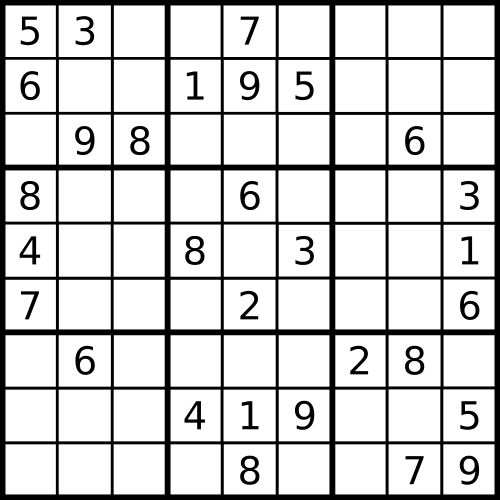
\includegraphics[width=.5\textwidth]{ex-sudoku.png}
  \caption{Exemple de grille de sudoku}%
  \label{fig:ex-sudoku}%
\end{figure}

Le programme devra accepter un paramètre passé en ligne de commande:
\begin{lstlisting}[style={},style=sh]
./sudoku path_to_sudoku_file
\end{lstlisting}
où \shell{path_to_sudoku_file} est le chemin d'accès à un fichier
texte au format sudoku (au sens expliqué ci-dessus). L'éxécution devra
alors renvoyer à l'écran la liste des solutions. Si plusieurs
solutions existent, elles devront être affichées, chacune au format
sudoku, avec une ligne vide les séparant.

\begin{remark}
  {\bf Attention} de bien respecter ces conventions, une partie de la
  correction étant automatisée: un petit programme de mon cru testera
  votre programme sur un grand nombre de sudokus et comparera le
  résultat à un fichier test contenant les solutions. Tout manquement
  aux conventions peut donc se solder à un échec du test même si votre
  algorithme est juste en soi!
\end{remark}

\medskip

L'implémentation de l'algorithme élaboré dans les parties
\ref{sec:exact-hit} à \ref{sec:dlx} et le respect des règles décrites
ci-dessus est le {\em strict minimum}. C'est-à-dire que tout
manquement aux prérogatives précédentes se ressentira drastiquement
dans la note. En particulier, on insiste sur le fait que le projet
rendu doit suivre l'algorithme décrit précédemment! Bien entendu, de
petites améliorations peuvent être apportées ici et là, mais le coeur
de l'algorithme doit rester celui développé en partie
\ref{sec:algo-sol}. Par exemple, un projet résolvant la grille de
sudoku par {\em brute-force} sera automatiquement écarté.

Ceci étant dit, le passage des prérogatives de cette seciton n'est pas
synonyme d'une note fixée : le code lui-même sera partie intégrante de
l'évaluation (un code concis, clair et élégant sera toujours préféré à
un code brouillon et peu lisible même si la sémantique des programmes
résultants est la même). {\bf Dans tous les cas, un code non commenté
  sera grandement pénalisé.}

\medskip

Enfin, toute amélioration du programme sera vivement appréciée et
pourra se voir attribuer des {\em points bonus}. Voici une liste
non-exhaustive de personnalisations possibles:
\begin{itemize}
\item proposer à l'utilisateur de rentrer la grille de sudoku à
  résoudre lignes à lignes en mode intéractif,
\item accepter un format plus large de grille de sudoku en entrée,
\item créer automatiquement des grilles de sudoku certifiées valides
  (i.e. dont on est sûr, grâce au solveur, qu'elles admettent une
  unique solution),
\item proposer de résoudre d'autres problèmes de satifaction de
  contraintes que le sudoku,
\item proposer un mode {\em verbose} qui montre toutes les étapes de
  résolution (attention, cela peut vite rendre la sortie indigeste
  pour l'utilisateur),
\item proposer {\bf en plus} un mode {\em brute-force} permettant de
  comparer le temps de calcul avec la méthode implémentée,
\item etc.
\end{itemize}
Pour être évaluée, toute amélioration devra venir avec un
documentation (interne ou externe au programme). Elle devra aussi être
compatible à la {\em version standard}: c'est-à-dire que si l'on fait
abstraction des améliorations, le programme doit fonctionner {\bf
  exactement} comme décrit dans les prérogatives à remplir. Un
manquement à cette dernière règle se verrait très pénalisé, puisque le
{\em strict minimum} ne serait alors pas atteint.

\bigskip

Le projet est à rendre pour le 14 janvier 2017. Vous êtes bien entendu
invités à collaborer à plusieurs dans votre réflexion, comme sur
n'importe quel devoir maison. En revanche, le projet final doit être
fait seul ou en binôme. Nous recommandons vivement l'option binôme: la
collaboration (souvent à bien plus que deux) est souvent de mise dans
les projets informatiques {\em de la vie réelle}. On conseille alors
d'utiliser un logiciel de {\em subversionning} pour vous simplifier la
tâche: les plus courant sont \shell{git}, \shell{svn} et
\shell{mercure}.

\end{document}